% abtex2-modelo-artigo.tex, v-1.9.2 laurocesar
% Copyright 2012-2014 by abnTeX2 group at http://abntex2.googlecode.com/ 
%

% ------------------------------------------------------------------------
% ------------------------------------------------------------------------
% abnTeX2: Modelo de Artigo Acadêmico em conformidade com
% ABNT NBR 6022:2003: Informação e documentação - Artigo em publicação 
% periódica científica impressa - Apresentação
% ------------------------------------------------------------------------
% ------------------------------------------------------------------------

\documentclass[
    % -- opções da classe memoir --
    article,            % indica que é um artigo acadêmico
    11pt,               % tamanho da fonte
    oneside,            % para impressão apenas no verso. Oposto a twoside
    a4paper,            % tamanho do papel. 
    % -- opções da classe abntex2 --
    %chapter=TITLE,     % títulos de capítulos convertidos em letras maiúsculas
    %section=TITLE,     % títulos de seções convertidos em letras maiúsculas
    %subsection=TITLE,  % títulos de subseções convertidos em letras maiúsculas
    %subsubsection=TITLE % títulos de subsubseções convertidos em letras maiúsculas
    % -- opções do pacote babel --
    english,            % idioma adicional para hifenização
    brazil,             % o último idioma é o principal do documento
    sumario=tradicional
    ]{abntex2}


% ---
% PACOTES
% ---

% ---
% Pacotes fundamentais 
% ---
\usepackage{lmodern}            % Usa a fonte Latin Modern
\usepackage[T1]{fontenc}        % Selecao de codigos de fonte.
\usepackage[utf8]{inputenc}     % Codificacao do documento (conversão automática dos acentos)
\usepackage[num,overcite]{abntex2cite}

\usepackage{indentfirst}        % Indenta o primeiro parágrafo de cada seção.
\usepackage{nomencl}            % Lista de simbolos
\usepackage{color}              % Controle das cores
\usepackage{graphicx}           % Inclusão de gráficos
\usepackage{microtype}          % para melhorias de justificação
\usepackage{listings}           % formatar codigo fonte http://linorg.usp.br/CTAN/macros/latex/contrib/listings/listings.pdf
% ---
        
% ---
% Pacotes adicionais, usados apenas no âmbito do Modelo Canônico do abnteX2
% ---
\usepackage{lipsum}             % para geração de dummy text
% ---
        
% ---
% Pacotes de citações
% ---
\usepackage[brazilian,hyperpageref]{backref}     % Paginas com as citações na bibl
\usepackage[num]{abntex2cite}   % Citações padrão ABNT
\usepackage[strings]{underscore}
% ---

% ---
% Configurações do pacote backref
% Usado sem a opção hyperpageref de backref
\renewcommand{\backrefpagesname}{Citado na(s) página(s):~}
% Texto padrão antes do número das páginas
\renewcommand{\backref}{}
% Define os textos da citação
\renewcommand*{\backrefalt}[4]{
    \ifcase #1 %
        Nenhuma citação no texto.%
    \or
        Citado na página #2.%
    \else
        Citado #1 vezes nas páginas #2.%
    \fi}%
% ---

% ---
% Informações de dados para CAPA e FOLHA DE ROSTO
% ---
\titulo{Construindo um Smart IoT Gateway}
\autor{Danilo Guimarães \thanks{guimaraesdjl@gmail.com} \and Ricardo Rodrigues \thanks{ricardo.faria@outlook.com.br} \and Uillan Araújo \thanks{uillan@outlook.com}}
\local{Brasil}
\instituicao{Centro Universitário Alves Faria}
\data{15 de Setembro de 2017}




% ---

% ---
% Configurações de aparência do PDF final

% alterando o aspecto da cor azul
\definecolor{blue}{RGB}{41,5,195}

% informações do PDF
\makeatletter
\hypersetup{
        %pagebackref=true,
        pdftitle={\@title}, 
        pdfauthor={\@author},
        pdfsubject={\@title},
        pdfcreator={LaTeX with abnTeX2},
        pdfkeywords={abnt}{latex}{abntex}{abntex2}{atigo científico}, 
        colorlinks=true,            % false: boxed links; true: colored links
        linkcolor=blue,             % color of internal links
        citecolor=blue,             % color of links to bibliography
        filecolor=magenta,              % color of file links
        urlcolor=blue,
        bookmarksdepth=4
}
\makeatother
% --- 

% ---
% compila o indice
% ---
\makeindex
% ---

% ---
% Altera as margens padrões
% ---
\setlrmarginsandblock{3cm}{3cm}{*}
\setulmarginsandblock{3cm}{3cm}{*}
\checkandfixthelayout
% ---

% --- 
% Espaçamentos entre linhas e parágrafos 
% --- 

% O tamanho do parágrafo é dado por:
\setlength{\parindent}{1.3cm}

% Controle do espaçamento entre um parágrafo e outro:
\setlength{\parskip}{0.2cm}  % tente também \onelineskip

% Espaçamento simples
\SingleSpacing

% ----
% Início do documento
% ----
\begin{document}

% Retira espaço extra obsoleto entre as frases.
\frenchspacing 

% ----------------------------------------------------------
% ELEMENTOS PRÉ-TEXTUAIS
% ----------------------------------------------------------

%---
%
% Se desejar escrever o artigo em duas colunas, descomente a linha abaixo
% e a linha com o texto ``FIM DE ARTIGO EM DUAS COLUNAS''.
% \twocolumn[           % INICIO DE ARTIGO EM DUAS COLUNAS
%
%---
% página de titulo
\maketitle

% resumo em português
\begin{resumoumacoluna}
 De acordo com o grande avanço da Computação, torna-se comum a coexistência de objetos reais com o mundo virtual. Devido a essa evolução, têm-se a necessidade de uma padronização de conceitos como a \textit{Internet of Things} (IoT) com a comunicação de seus dispositivos, assim surge a ideia de um Gateway para agregar e centralizar essa transição de informações. Este trabalho propõe um estudo breve sobre Gateway IoT, isto é, construir um software Smart IoT Gateway funcional e utilizável em projetos de pequeno e médio porte.
 \vspace{\onelineskip}
 
 \noindent
 \textbf{Palavras-chaves}: Internet of Things. IoT Gateway. Arquitetura de Software.
\end{resumoumacoluna}

\renewcommand{\resumoname}{Abstract}
\begin{resumoumacoluna}
	\begin{otherlanguage*}{english}
		According to the great advance of Computing, it becomes common the coexistence of real objects with the virtual world. Due to this evolution, there is a need for a standardization of concepts such as Internet of Things (IoT) with the communication of its devices, thus the idea of a Gateway to aggregate and centralize this transition of information. Thus, this work proposes a brief study on Gateway IoT, that is, to build an Smart IoT Gateway functional and usable in small and medium-sized projects.
		\vspace{\onelineskip}
		\noindent
		
		\textbf{Key-words}: Internet of Things. IoT Gateway. Software Architecture.
	\end{otherlanguage*}  
\end{resumoumacoluna}

% ]                 % FIM DE ARTIGO EM DUAS COLUNAS
% ---

% ----------------------------------------------------------
% ELEMENTOS TEXTUAIS
% ----------------------------------------------------------
\textual

% ----------------------------------------------------------
%% CAPITULOS
% ----------------------------------------------------------


\chapter{Introdu��o}
\label{cap:intro}

Este documento mostra como usar o \LaTeX\ com a classe \textsf{inf-ufg} para formatar teses, disserta��es, monografias e relat�rios de conclus�o de curso, segundo o padr�o adotado pelo Instituto de Inform�tica da UFG. Este documento e a classe \textsf{inf-ufg} foram, em grande parte, copiados e adaptados da classe \textsf{thesisPUC} e do texto de Thomas Lewiner \cite{Lew2002} que descreve a sua utiliza��o.

 \LaTeX\ � um sistema de editora��o eletr�nica muito usado para produzir documentos cient�ficos de alta qualidade tipogr�fica. O sistema tamb�m � �til para produzir todos os tipos de outros documentos, desde simples cartas at� livros completos.

Se voc� precisar de algum material de apoio referente ao \LaTeX, d� uma olhada em um dos sites do Comprehensive TEX Archive Network (CTAN). O site est� em \href{http://www.ctan.org/}{www.ctan.org}. Todos os pacotes podem ser obtidos via \textsf{FTP} \href{ftp://www.ctan.org/}{ftp://www.ctan.org} e existem v�rios servidores em todo o mundo. Eles podem ser encontrados, por exemplo, em \href{ftp://ctan.tug.org/}{ftp://ctan.tug.org} (EUA), \href{ftp://ftp.dante.de/}{ftp://ftp.dante.de} (Alemanha), \href{ftp://ftp.tex.ac.uk/}{ftp://ftp.tex.ac.uk} (Reino Unido).

Voc� pode encontrar uma grande quantidade de informa��es e dicas na p�gina dos usu�rios brasileiros de \LaTeX\ (\TeX-BR). O endere�o � \href{http://biquinho.furg.br/tex-br/}{http://biquinho.furg.br/tex-br/}.
Tanto no CTAN quanto no \TeX-BR est�o dispon�veis bons documentos em portugu�s sobre o \LaTeX. Em particular no CTAN, est� dispon�vel uma introdu��o bastante completa em portugu�s: \href{http://www.ctan.org/tex-archive/info/lshort/portuguese-BR/lshortBR.pdf}{CTAN:/tex-archive/info/lshort/portuguese-BR/}. No \TeX-BR tamb�m existe um documento com exemplos de uso de \LaTeX\ e de v�rios pacotes: \href{http://biquinho.furg.br/tex-br/doc/LaTeX-demo/}{http://biquinho.furg.br/tex-br/doc/LaTeX-demo/} . O objetivo � ser, atrav�s de exemplos, um guia para o usu�rio de \LaTeX\ iniciante e intermedi�rio, podendo, ainda, servir como um guia de refer�ncia r�pida para usu�rios avan�ados.

Se voc� quer usar o \LaTeX\ em seu computador, verifique em quais sistemas ele est� dispon�vel em \href{http://www.ctan.org/tex-archive/systems/}{CTAN:/tex-archive/systems}. Em particular para \textsf{MS Windows}, o sistema gratuito \href{http://www.miktex.org/}{MikTeX}, dispon�vel no CTAN e no site \href{http://www.miktex.org/}{www.miktex.org} � completo e atualizado de todas as op��es  que voc� poderia precisar para editar o seu texto.

O estilo \textsf{inf-ufg} se integra completamente ao \LaTeXe. Uma tese, disserta��o ou monografia escrita no estilo padr�o do \LaTeX\ para teses (estilo \verb|report|) pode ser formatada em 15 minutos para se adaptar �s normas da UFG.

O estilo \textsf{inf-ufg} foi desenhado para minimizar a quantidade de texto e de comandos necess�rios para escrever a sua disserta��o. S� � preciso inserir algumas macros no in�cio do seu arquivo \LaTeX, precisando os dados bibliogr�ficos da sua disserta��o (por exemplo o seu nome, o titulo da disserta��o\ldots). Em seguida, cada p�gina dos elementos pr�-textuais ser� formatada usando macros ou ambientes espec�ficos. O corpo do texto � editado normalmente. Finalmente, as refer�ncias bibliogr�ficas podem ser entradas manualmente (via o comando \verb|\bibitem| do \LaTeX\ padr�o) ou usando o sistema BiBTeX (muito mais recomend�vel). Neste caso, os arquivos \verb|inf-ufg.bst| e \verb|abnt-alf.bst| permitem a formata��o das refer�ncias bibliogr�ficas segundo as normas da UFG.


\section{Internet of Things}
\label{sec:iot}

A Internet começou como uma forma do governo comunicar após uma guerra nuclear, mas evoluiu para ser muito mais do que uma rede. De muitas maneiras, a Internet tornou-se um mundo digital que tem ligações ao nosso mundo físico \cite{BrasilEscola}.

Conforme as tecnologias avançam, torna-se cada vez mais comum que todos estejam conectados. E com essa evolução os objetos físicos passam a coexistir com a Internet, impactando em diversos aspectos no cotidiano das pessoas seja no profissional ou pessoal.

A Internet das Coisas (do inglês, \textit{Internet of Things}, ou simplesmente IoT) é essa revolução tecnológica que visa conectar dispositivos eletrônicos (como aparelhos eletrodomésticos, máquinas industriais, meios de transporte etc.) à Internet. IoT é um termo criado por Kevin Ashton \cite{Kevin}, um pioneiro da tecnologia britânico que concebeu, em 1999, um sistema de sensores onipresentes conectando o mundo físico à Internet, enquanto trabalhava em identificação por rádio frequência (RFID). O grande valor da IoT está no preenchimento das lacunas entre o mundo físico e digital em sistemas \cite{Amazon}.

Na sua essência, a IoT significa apenas um ambiente que reúne informações de vários dispositivos (computadores, smartphones, semáforos, e quaisquer coisa com um sensor) e de aplicações (qualquer coisa desde uma aplicação de mídia social como o Twitter a uma plataforma de comércio eletrônico, de um sistema de produção a um sistema de controlo de tráfego). Quando se combinam informações de dispositivos e de outros sistemas, enormes recursos de processamento são utilizados para análises expansivas, geralmente associadas com o conceito de \textit{Big Data} \footnote{\textit{Big Data} é um termo usado para referenciar grandes e complexos volumes de informações que necessitam de técnicas e ferramentas específicas para serem capturadas, gerenciadas e/ou processadas} – ou seja, a análise de dados não necessariamente concebidos para serem avaliados em conjunto. Esta noção de múltiplas finalidades é provavelmente a melhor razão para usar o termo “Internet das Coisas”, quando a Internet é mais do que uma rede resistente para ser um canal para qualquer combinação e coleção de atividades digitais \cite{ComputerWorld}.

Em seu processo evolutivo a IoT enfrenta diversos problemas, que variam de aplicativos (sistemas), politicas de segurança e até problemas técnicos. Com todos estes dispositivos conectados à Internet uma enorme quantidade de informação é disponibilizada levantando questões de confiabilidade destas informações. Onde e quem garantirá a autenticidade dessas informações? Quem pode ter acesso à essas informações? Quem irá proteger essas informações? São alguns dos problemas enfrentamos ao se disponibilizar as informações de objetos do mundo físico ao mundo virtual. Uma padronização entre as tecnologias é bastante importante, pois ela levará a uma melhor interoperabilidade, reduzindo barreiras. Muitos fabricantes estão criando suas próprias soluções (Intel, Dell etc.) o que as levam à ter comportamentos diferentes, dificultando a integração destes sistemas ou dispositivos \cite{IEEEORG, CMSWIRE}.
\section{IoT Gateway}
\label{sec:iotGateway}

Quando falamos de IoT, ou Internet das Coisas, já pensamos em que algo estará conectado à Internet. Essa “coisa” não necessariamente se conecta de forma direta, sendo, na grande maioria dos casos, por meio um gateway ou roteador.

O gateway é similar a um roteador, porém, ele pode unir redes de diferentes protocolos, através de um processamento local para a tradução e conversão de protocolos. Gateways são muito utilizados em ambiente industrial e corporativo, porém, com o avanço do IoT, está ficando mais comum encontrar esse tipo de equipamento para uso residencial.

A grande vantagem em fazer o seu próprio gateway, é o nível de customização que ele pode ter, já que temos total acesso ao sistema operacional, sem restrições impostas pelo fabricante – o que ocorre na maioria dos casos. Essa customização vai permitir usar o gateway em modo “fog computing” (computação em nevoeiro), para o processamento de informações o mais perto do dispositivo da borda, ou edge device, fazendo com que, mesmo na falta de Internet, o dispositivo consiga se manter operacional, ainda que com algumas restrições.

Fazer o seu próprio gateway de IoT pode parecer loucura, mas com a baixa nos preços dos SoC’s (System-on-a-Chip), alavancado principalmente pela Raspberry Pi, torna possível a criação de sistemas computacionais de bom desempenho, tamanho reduzido e baixo custo. Já é possível encontrar SoC’s custando menos de US$ 10.



-- Escrever direto sobre Gateway IOT
\section{Solução desenvolvida}
\label{sec:iotGateway}

Esta seção detalha os objetivos e decisões arquiteturais. Foi desenvolvida uma solução de software de \textit{Smart Gateway IoT} que está disponibilizada no Github, capaz de receber dados através de uma rede utilizando o protocolo MQTT	(\ref{mqtt}) de um dispositivo previamente cadastro e armazenar essas informações. Os dados recebidos são analisados para a estrutura que irá definir a execução ou não de um fluxo de notificação através de SMS (\ref{sms}) para um número definido.

\subsection{Tecnologias Utilizadas} 
\begin{itemize}
	\item Node.js \footnote{NodeJS - \url{https://nodejs.org/en/}} v6.x;
	\item TypeScript \footnote{Typescript - \url{http://www.typescriptlang.org/}} v2.3 com transpile para ES6;
	\item TSLint \footnote{TSLint - \url{https://palantir.github.io/tslint/}} v4.x com recomendações gerais padrão;
	\item Jest \footnote{Jest - \url{https://facebook.github.io/jest/}}para teste unitário e cobertura;
	\item AngularJS \footnote{AngularJS - \url{https://angularjs.org/}} v1.6 para o front end da aplicação ;
	\item MongoDB \footnote{MongoDB - \url{https://www.mongodb.com/}} para persistência;
	\item MQTT (\ref{mqtt}) como protocolo de comunicação entre os sensores e o Gateway;
	\item SMS (\ref{sms}) como serviço de mensageria;
	\item ExpressJS \footnote{ExpressJS - \url{http://expressjs.com/}} como framework web Node.js 
\end{itemize}

O Node.js foi escolhido por conta de seu baixo consumo de memória e processamento, além da sua característica de Non-Blocking IO \cite{NodeJSNonBlockingIO}, garantindo que possamos servir mais clientes com menos recursos, objetivo essencial para aplicações que podem ser executadas em um Raspberry Pi por exemplo.

A escolha pelo TypeScript \footnote{Typescript - \url{http://www.typescriptlang.org/}}, linguagem que é um superset do Javascript padrão foi motivada por garantir uma estrutura tipada, de forma que a manutenção do código fosse facilitada e as regras de negócio pudessem estar ligadas a um contrato de objeto.

Já o AngularJS \footnote{AngularJS - \url{https://angularjs.org/}} foi escolhido, por ser uma tecnologia que funciona com javascript nativo, sem necessidade de nenhum pós-processador para servir a aplicação aos clientes, permitindo o seu uso diretamente entre os arquivos estáticos do mesmo servidor Node.js que expõe a aplicação. Além disso, contou como um ponto para a escolha, a experiência prévia da equipe no desenvolvimento com esta tecnologia.

\subsubsection{Protocolos de comunicação}
\label{protocolos}

\phantomsection{SMS}\label{sms}, abreviação de \textit{Short Message Service}, é um serviço de troca de mensagens curtas de textos que permite o envio de mensagens para aparelhos celulares, conforme os padrões definidos no GSM (\textit{Global System for Mobile Communications}). Seu uso é bastante popular (cerca de 3,6 bilhões de usuários) \cite{SMS} e ubíquo (presente em praticamente qualquer país) \cite{SMSItu}. Além do que seu uso é fácil e barato, uma vez que o usuário receptor não requer conexão com a Internet para receber a mensagem, bastando possuir sinal com a rede de telefonia.

O \phantomsection{MQTT}\label{mqtt}, abreviação de \textit{Message Queue Telemetry Transport}, é um protocolo de comunicação altamente voltado para IoT. Ele foi arquitetado para ser um sistema de mensageria leve do tipo publisher/subscriber, para rodar em dispositivos limitados, tanto do ponto de vista da quantidade de memória para execução do programa, quanto do ponto de vista da conectividade. Redes lentas ou com alta latência não são problemas para esse protocolo. Geralmente, sensores IoT podem residir em locais extremamente hostis do ponto de vista de infra-estrutura de conexão de dados.

\subsection{Modelo de Dados}
O modelo de dados foi concebido com a intenção de tornar as etapas do processo altamente plugáveis e customizáveis no curto e longo prazo, garantindo as funcionalidades básicas do MVP \footnote{\textit{Minimum Viable Product}, ou Produto Mínimo Viável, é um termo utilizado para caracterizar um produto com as features necessárias para os primeiros clientes \cite{MVP}} executado e a possibilidade de extensibilidade no futuro com retrocompatibilidade. 

Nesta modelagem, a entidade \verb|Dispositivo| identifica um aparelho qualquer que se conecte ao gateway para transmitir informações, o aparelho deve definir um ID de conexão que é cadastrado nesta entidade. Com relação direta a entidade \verb|Dispositivo|, e a entidade \verb|Trigger| modela um gatilho clássico, composto de condição e ação. Nesta perspectiva, a condição é a entidade \verb|Operação| que permite avaliar os valores recebidos e identificar se eles são iguais ou estão no intervalo de valor definidos por esta entidade. A entidade \verb|Evento| por sua vez é a ação, onde é definido o que acontecerá caso a condição seja atendida, por exemplo, o envio de SMS para um destinatário com o determinado texto, ver Figura~\ref{fig:modeloDeDados}.

Além das entidades que servem diretamente a execução do fluxo principal da aplicação, temos 3 entidades de funções secundárias. \verb|Configuracao| é responsável por armazenar os dados utilizados para configurar a aplicação, como a configuração das credenciais para uso do serviço de SMS. As entidades \verb|HistoricoEvento| e \verb|HistoricoMensagem| são responsáveis por armazenar os dados recebidos e os eventos executados.

\begin{figure}[h!]
	\begin{center}
		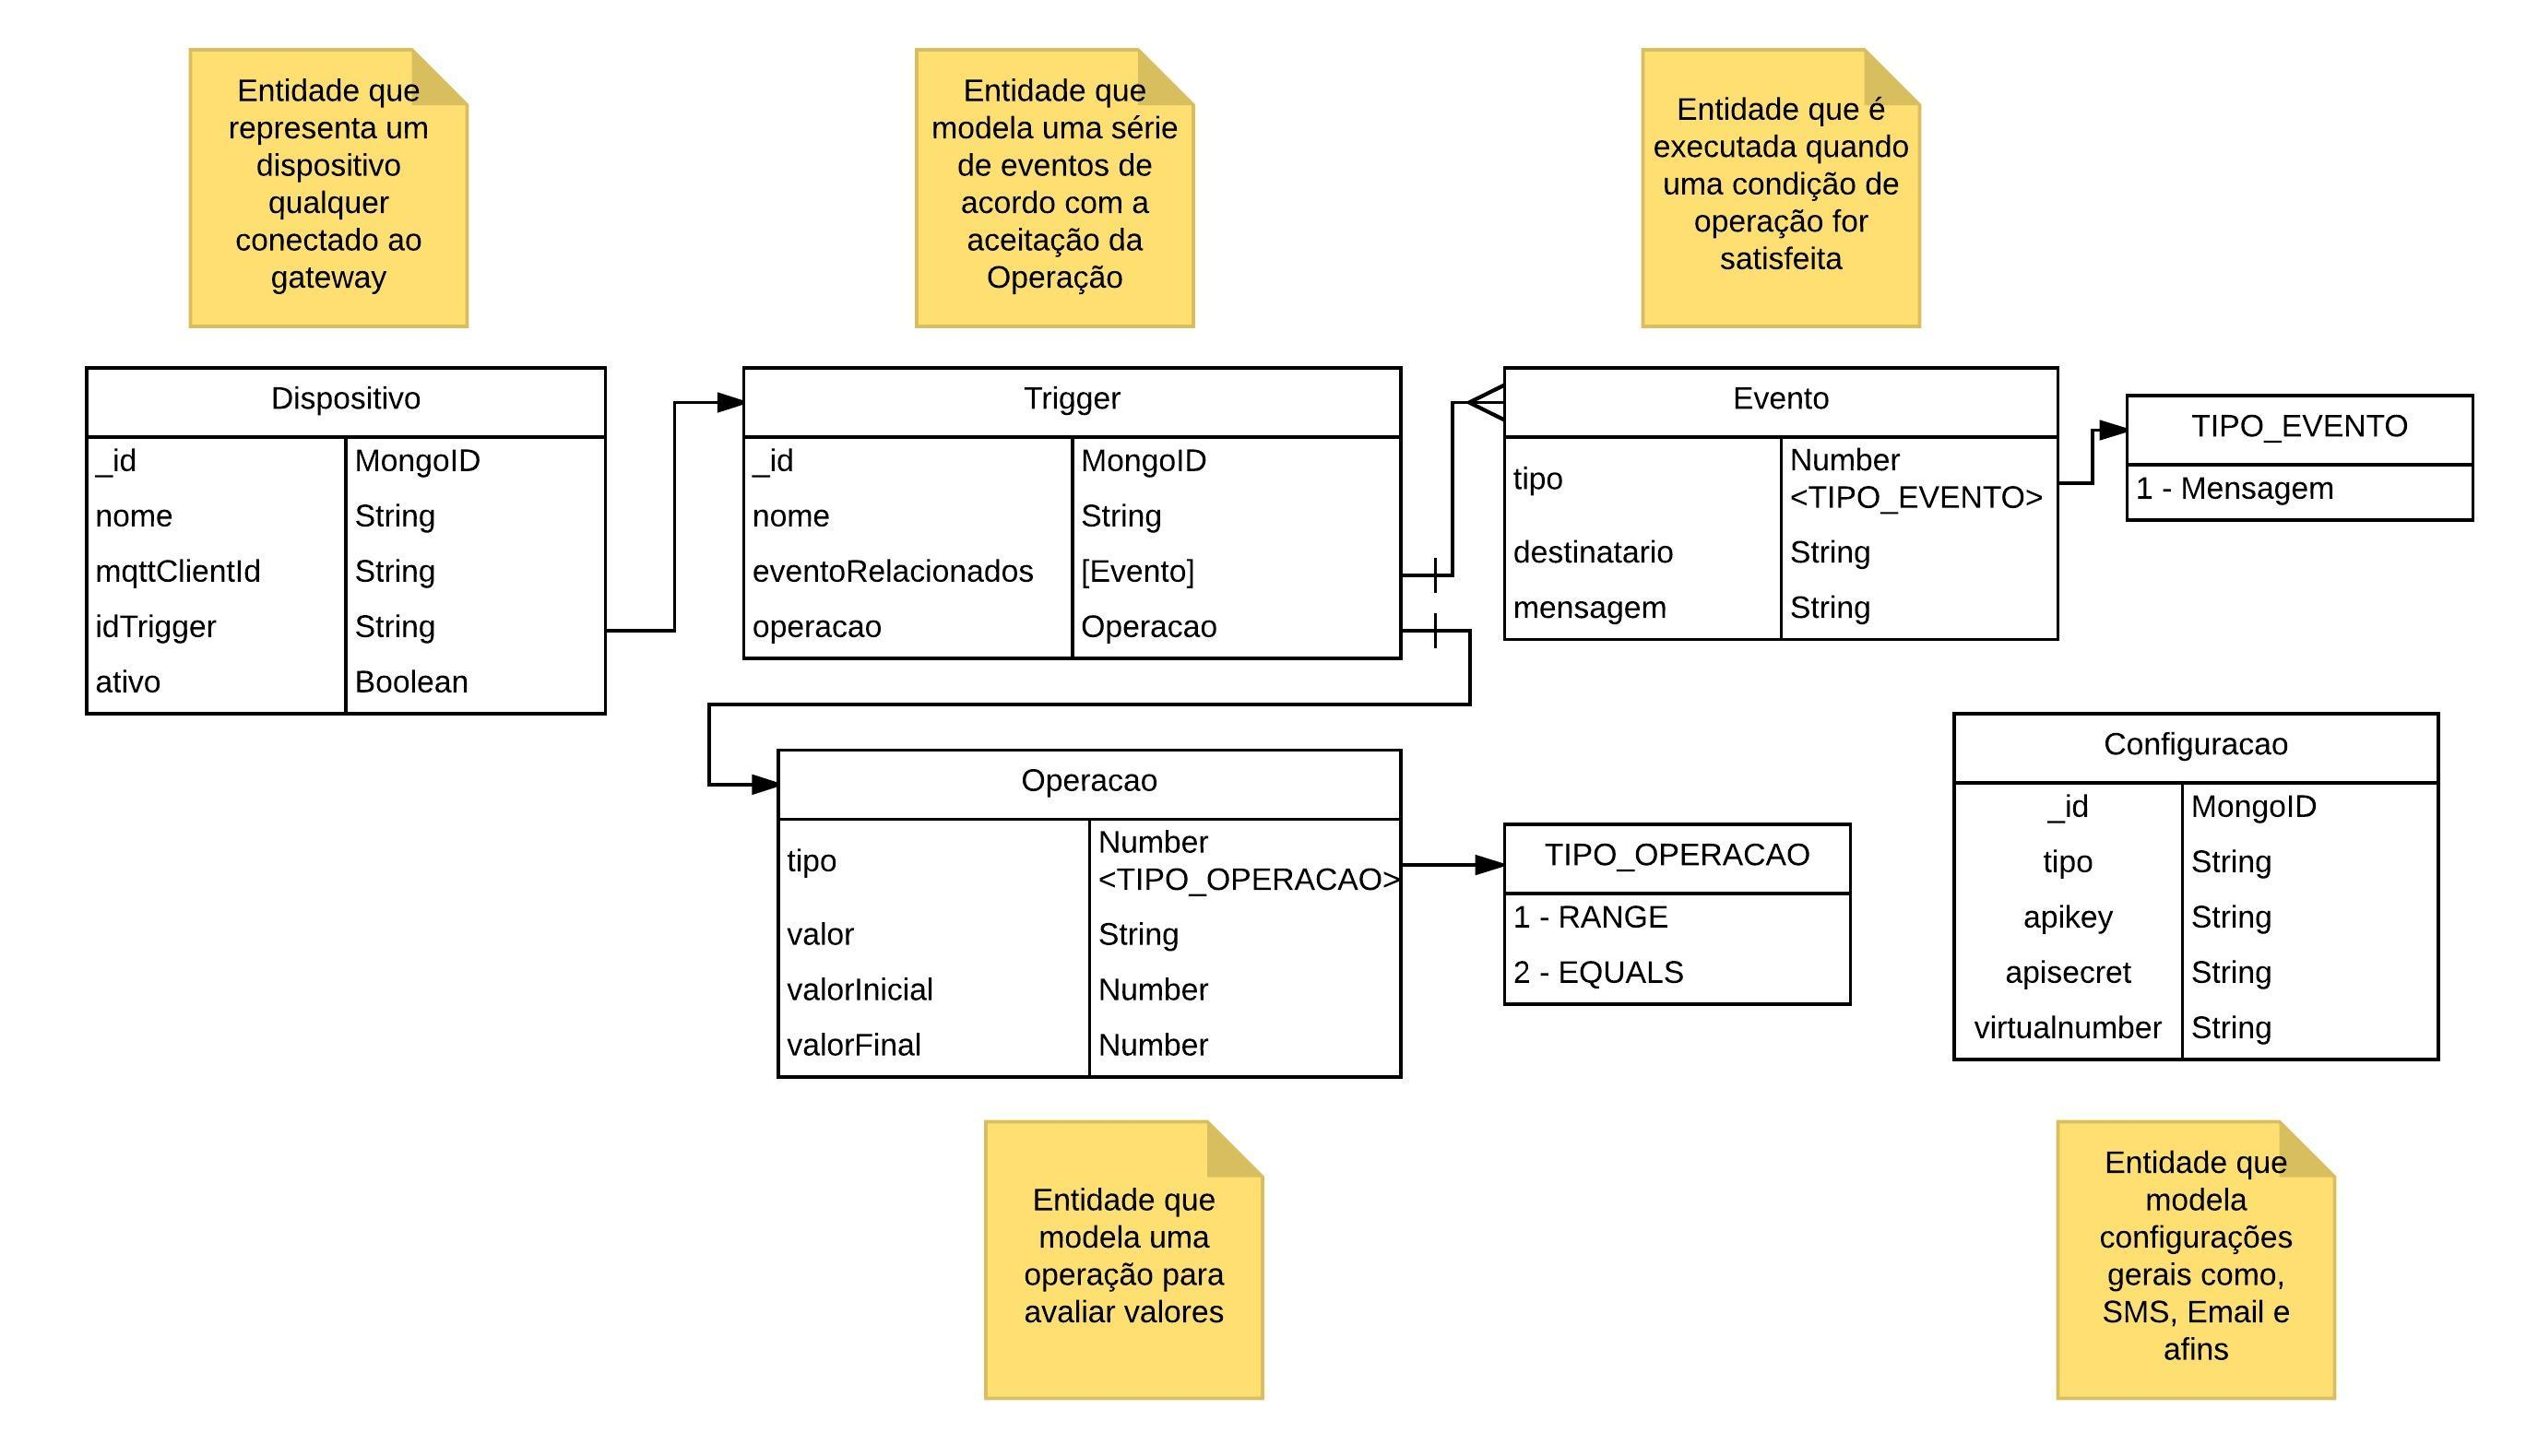
\includegraphics[width=1.085\textwidth]{./img/modelo-de-dados}
		\caption{Representação esquemática da modelagem de dados.}
		\label{fig:modeloDeDados}
	\end{center}
\end{figure}

\begin{figure}[h!]
		\begin{center}
		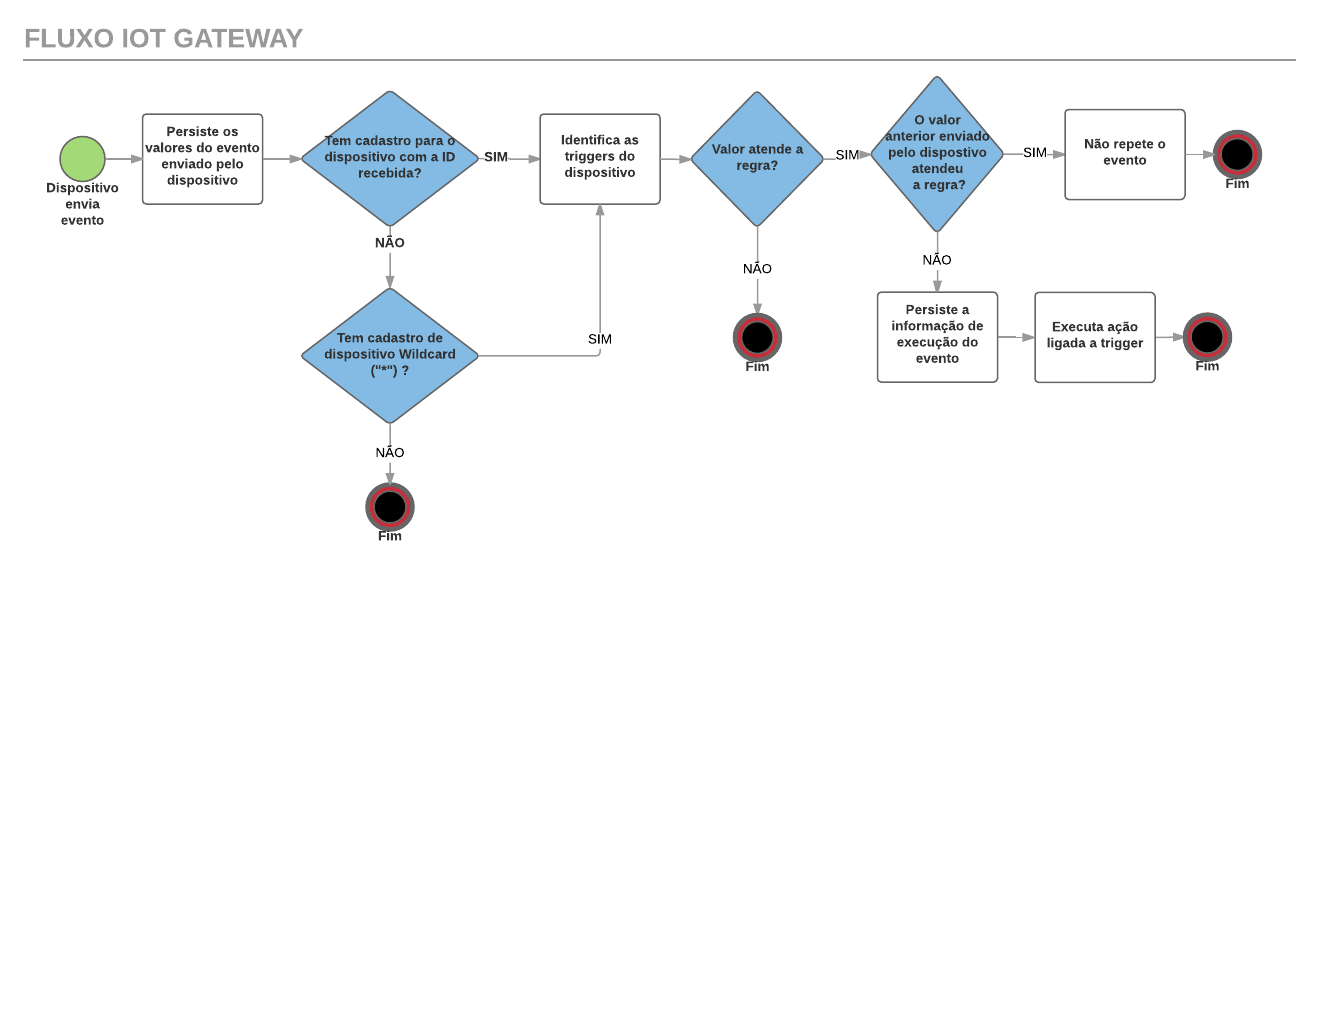
\includegraphics[width=0.9\textwidth]{./img/fluxograma}
		\caption{Representação esquemática do fluxo Gateway IoT.}
		\label{fig:fluxograma}
	\end{center}
\end{figure}

A modelagem desenvolve uma estrutura sequencial que parte da identificação do dispositivo, análise dos gatilhos ligados a este dispositivo, avaliação da operação lógica e liberação para execução do evento, ver Figura~\ref{fig:fluxograma}.  

\subsection{Requisitos funcionais}
\label{reqFuncionais}

Os requisitos funcionais levados em consideração nesse trabalho foram:

\begin{itemize}
	\item Requisito 1: Envio de mensagens via SMS \cite{SMS}
	
	\item Requisito 2: Cadastro de número de celular.
\end{itemize}

\subsection{Requisitos não funcionais}
\label{reqNaoFuncionais}

Requisitos não funcionais, como os de extensibilidade e de retrocompatibilidade, agregam muito esforço no desenho de um MVP, mas são aspectos que em hipótese alguma podem ser desconsiderados.
\section{Resultados}
\label{sec:resultados}

Como resultados deste trabalho, podemos destacar o fomento à discussão de soluções que tornem o desenvolvimento para IoT mais simples, removendo a necessidade de codificação de softwares para receber os eventos para cada projeto, conseguindo resultados em um menor tempo. E como principal ponto o desenvolvimento do software que atenda requisitos de um gateway, performático e portável, abaixo demonstraremos algumas imagens do sistema funcionando.

Na Figura~\ref{fig:raspberryDistroRaspbian} pode-se observar a aplicação sendo inicializada em um Raspberry Pi 3 Model B v1.2 (ver Figura~\ref{fig:raspberryPi3ModelB}), onde a porta TCP 3000 escutará as requisições Web e a porta TCP 1885 onde os dispositivos se conectarão pelo protocolo MQTT.
\begin{figure}[h!]
	\begin{center}
		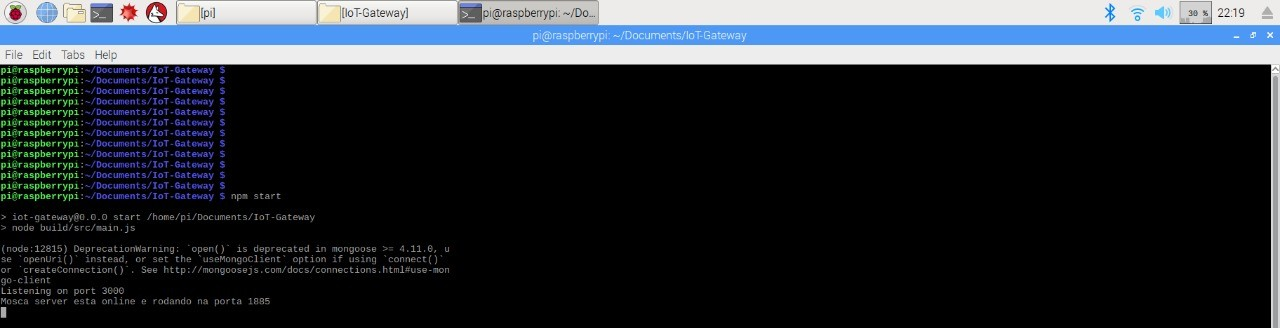
\includegraphics[width=1.085\textwidth]{./img/raspberryDistroRaspbian}
		\caption{Representação execução aplicação.}
		\label{fig:raspberryDistroRaspbian}
	\end{center}
\end{figure}

\begin{figure}[h!]
	\begin{center}
		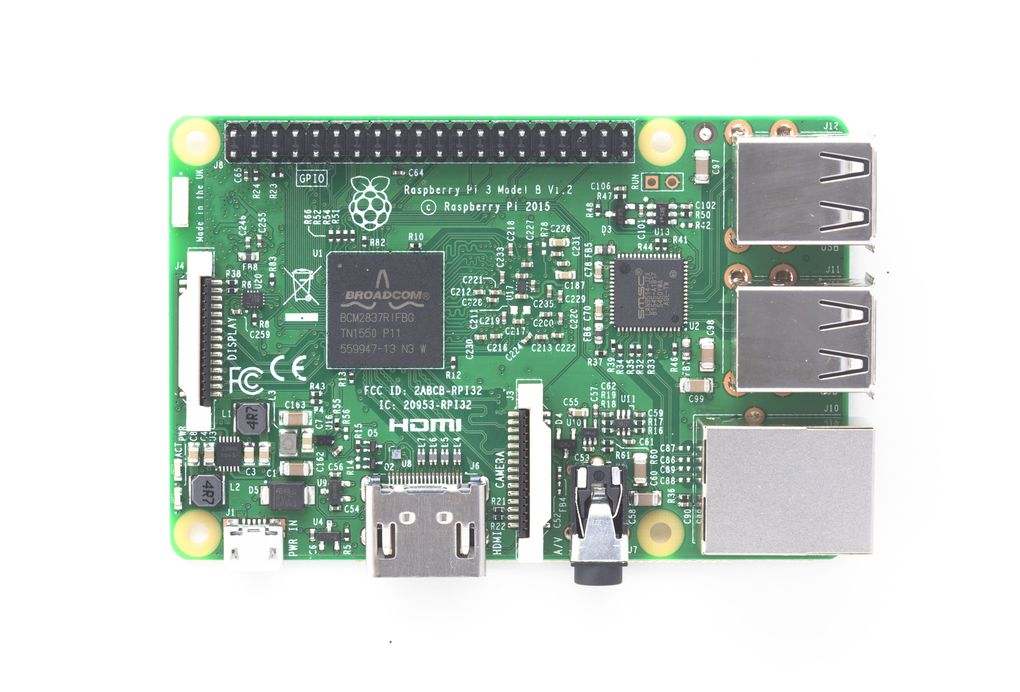
\includegraphics[width=1.085\textwidth]{./img/raspberry-pi-3}
		\caption{Exemplar do \textit{Raspberry Pi 3 Model B v1.2}, o SoC utilizado nesse trabalho}
		\label{fig:raspberryPi3ModelB}
	\end{center}
\end{figure}

Na Figura~\ref{fig:dadosBasicos} temos a tela inicial da aplicação com algumas informações a respeito da aplicação.
\begin{figure}[h!]
	\begin{center}
		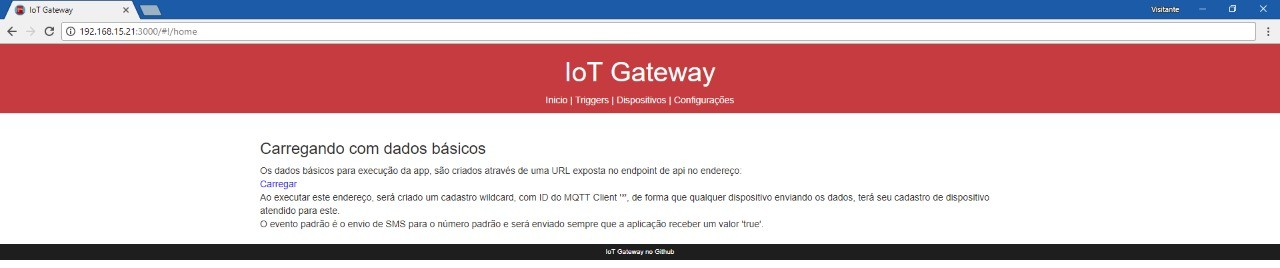
\includegraphics[width=1.085\textwidth]{./img/dadosBasicos}
		\caption{Representação visual da tela dos dados básicos.}
		\label{fig:dadosBasicos}
	\end{center}
\end{figure}

Na Figura~\ref{fig:triggerCadastrada} vemos o cadastro de uma \textit{trigger} com operação lógica de intervalo, onde o evento será executado apenas caso o valor enviado pelo dispositivo esteja entre 1 e 10. Um cenário claro de uso desta funcionalidade seria o uso do gateway para enviar notificações caso um sensor leia informações de um cenário crítico.
\begin{figure}[h!]
	\begin{center}
		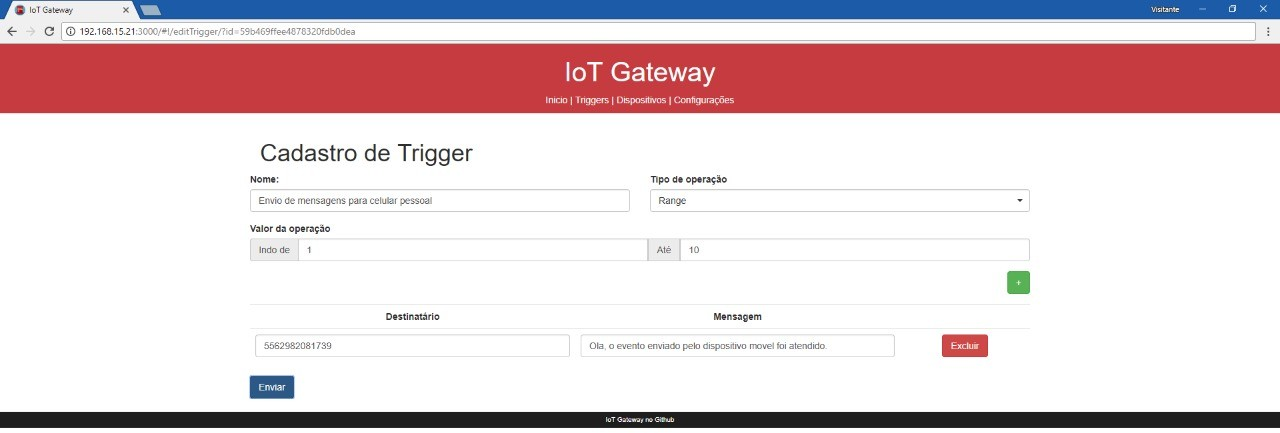
\includegraphics[width=1.085\textwidth]{./img/triggerCadastrada}
		\caption{Representação visual da tela de cadastro de trigger.}
		\label{fig:triggerCadastrada}
	\end{center}
\end{figure}

Na Figura~\ref{fig:dispositivoCadastrado} temos a listagem de dispositivos cadastrados, onde o dispositivo de nome \verb|"Celular com MyMqtt"| está cadastrado, mas sua identificar é \verb|"*"| que permite que qualquer dispositivo seja identificado por este cadastrado.
\begin{figure}[h!]
	\begin{center}
		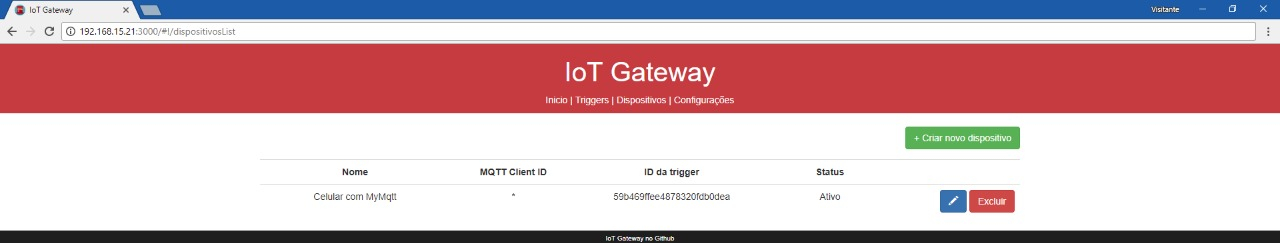
\includegraphics[width=1.085\textwidth]{./img/dispositivoCadastrado}
		\caption{Representação visual da tela de cadastro de dispositivos.}
		\label{fig:dispositivoCadastrado}
	\end{center}
\end{figure}

Na Figura~\ref{fig:aplicativoAndroidMQTT} temos um dispositivo android conectado ao gateway utilizando MQTT e enviando eventos para análise.
\begin{figure}[h!]
	\begin{center}
		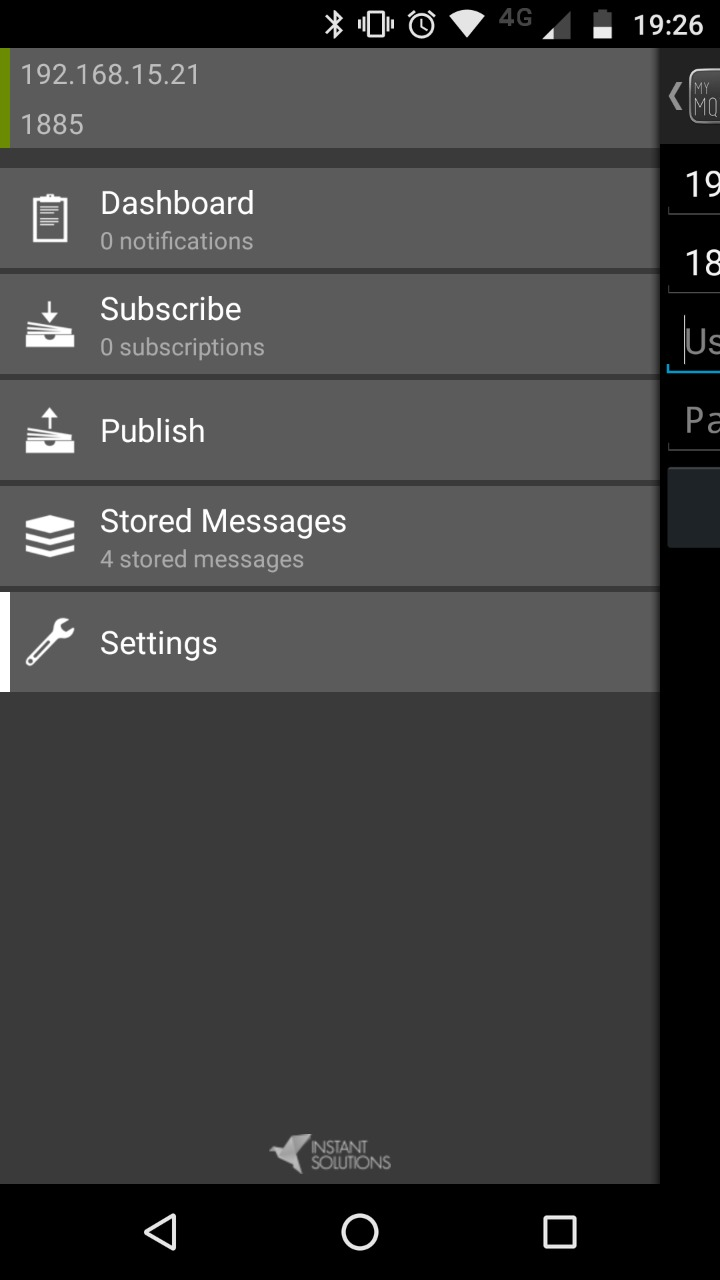
\includegraphics[width=0.85\textwidth]{./img/aplicativoAndroidMQTT}
		\caption{Representação visual do dispositivo Android utilizando protocolo MQTT.}
		\label{fig:aplicativoAndroidMQTT}
	\end{center}
\end{figure}

Na Figura~\ref{fig:eventoConsole} visualizamos o log da aplicação de 2 eventos, um em que o cenário não foi atendido, e outro em seguida onde o mesmo foi atendido e enviou o SMS.
\begin{figure}[h!]
	\begin{center}
		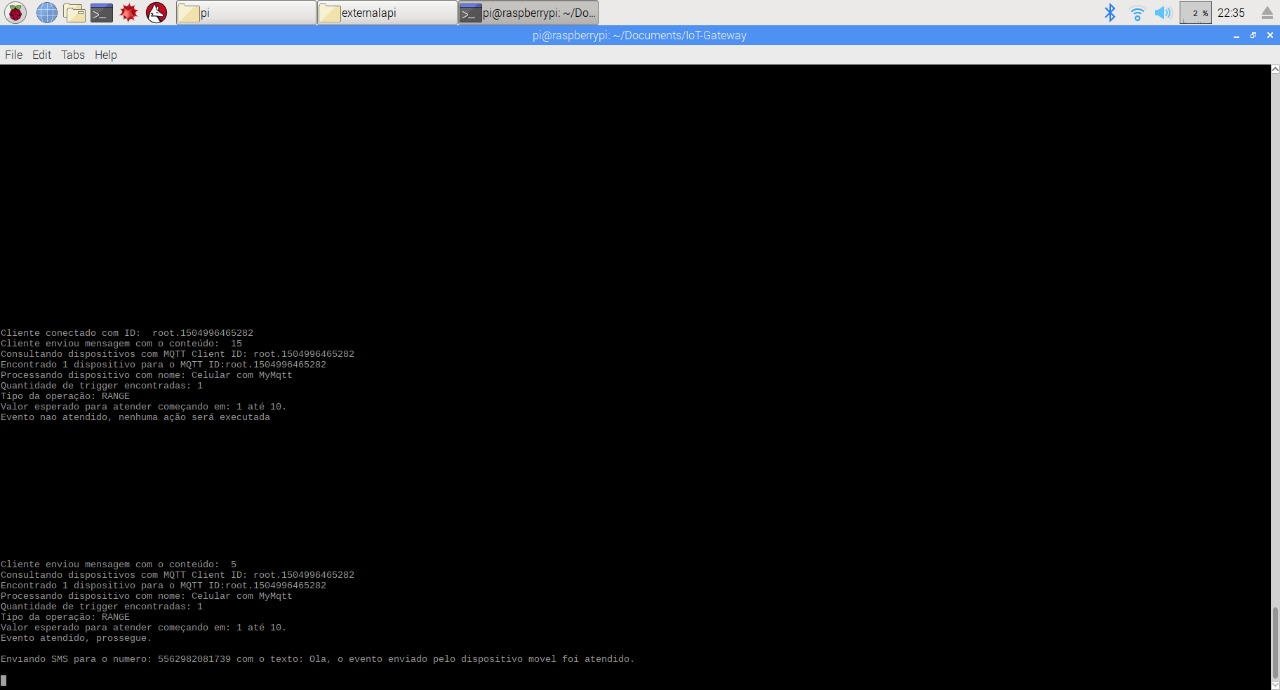
\includegraphics[width=1.085\textwidth]{./img/eventoAtendidoNaoAtendidoConsole}
		\caption{Representação visual do console ao receber eventos.}
		\label{fig:eventoConsole}
	\end{center}
\end{figure}

Na Figura~\ref{fig:smsRecebido2} o SMS recebido pelo celular após o evento atendido.
\begin{figure}[h!]
	\begin{center}
		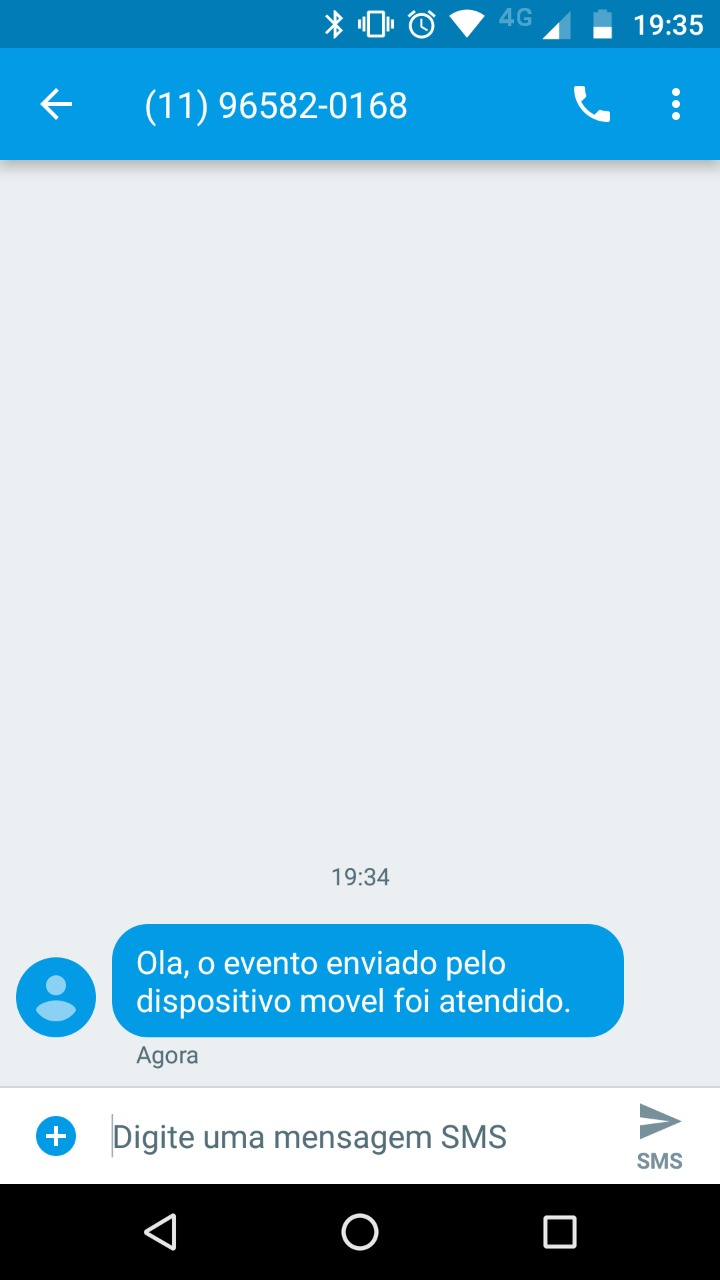
\includegraphics[width=0.8\textwidth]{./img/smsRecebido2}
		\caption{Representação visual do SMS recebido.}
		\label{fig:smsRecebido2}
	\end{center}
\end{figure}

Todos os eventos atendidos e dados recebidos são armazenados no banco de dados da aplicação para consulta posterior.


% ---
% Finaliza a parte no bookmark do PDF, para que se inicie o bookmark na raiz
% ---
\bookmarksetup{startatroot}% 
% ---

% ---
% Conclusão
% ---
\section*{Considerações finais}
\addcontentsline{toc}{section}{Considerações finais}

Durante o desenvolvimento desse trabalho, podemos concluir que a possibilidade de soluções usando IoT é extremamente vasta e extensa. A indústria, como um todo, está aquecida e pretende absorver toda gama de demanda de eventuais serviços que envolvam esse tipo de tecnologia.

Por se tratar de um ramo da Computação que é relativamente novo (o termo foi cunhado em 1999 \cite{Kevin}, somando assim apenas 18 anos de idade no momento que este trabalho é publicado), alguns termos e definições não possuem uma consistência desejável e costumam divergir muito de autor para autor. O que caracteriza um certo aspecto positivo, tal que ainda há muito espaço para que mais trabalhos possam ser feitos e consolidados na indústria de IoT.

Existem tecnologias Web modernas, principalmente as baseadas em Javascript, que propiciam a construção de softwares voltado para IoT de forma fácil, produtiva, testável e manutenível.

Na elaboração desse projeto, no que tange a perspectiva da escrita do software, podemos dizer que o maior desafio foi dos pontos de vista da elaboração arquitetural e de modelagem de dados, de forma que após as definições, a escrita do código foi relativamente simples. Requisitos não funcionais, como os de extensibilidade e de retrocompatibilidade, agregam muito esforço no desenho de um MVP, mas são aspectos que em hipótese alguma podem ser desconsiderados.




% ----------------------------------------------------------
% ELEMENTOS PÓS-TEXTUAIS
% ----------------------------------------------------------
\postextual

% ----------------------------------------------------------
% Referências bibliográficas
% ----------------------------------------------------------
\clearpage
\bibliography{./bib/artigo}

% ----------------------------------------------------------
% Glossário
% ----------------------------------------------------------
%
% Há diversas soluções prontas para glossário em LaTeX. 
% Consulte o manual do abnTeX2 para obter sugestões.
%
%\glossary

% ----------------------------------------------------------
% Apêndices
% ----------------------------------------------------------

% ---
% Inicia os apêndices
% ---
\clearpage
%\begin{apendicesenv}

% ----------------------------------------------------------
\chapter{Nullam elementum urna vel imperdiet sodales elit ipsum pharetra ligula
ac pretium ante justo a nulla curabitur tristique arcu eu metus}
% ----------------------------------------------------------
\lipsum[55-57]

\end{apendicesenv}



% ----------------------------------------------------------
% Anexos
% ----------------------------------------------------------
\cftinserthook{toc}{AAA}
% ---
% Inicia os anexos
% ---
%\anexos
%\begin{anexosenv}

% ---
\chapter{Cras non urna sed feugiat cum sociis natoque penatibus et magnis dis
parturient montes nascetur ridiculus mus}
% ---

\lipsum[31]

\end{anexosenv}

\end{document}